\chapter{Latent ODE and SDE models}\label{sec:Latent ODE and SDE models}

\section{Latent ODE models}

\glspl{latent ode} is a class of models introduced in \cite{chen_neural_2019} : "Neural Ordinary Differential Equations" 
by Ricky T. Q. Chen, Yulia Rubanova, Jesse Bettencourt, David Duvenaud. 
ArXiV : \href{https://arxiv.org/abs/1806.07366}{Neural ODE Best Paper Award NeurIPS 2018}.\\

The starting point is to write the evolution of the latent state $z_t$ as:
\begin{align}
    z_{t+1} &= z_t + f(z_t, \theta_t)
\end{align}
where $z_t \in \mathbb{R}^D$ is the latent state, $\theta_t$ is a set
 of parameters at time $t$, and $f$ is a function.

This formulation is the one used in ResNet blocks, and can be 
seen as the Euler transformation of a continuous transformation.

Taking the expression to the limit as $dt \rightarrow 0$, we can write an 
\gls{ode}:
\begin{align}
    \frac{dz_t}{dt} &= f(z_t, t, \theta_f)
\end{align}
where $\theta_f$ is a set of parameters, that can typically be the parameters of 
a neural network learning $f$.

For a time series $x_{t_1}, x_{t_2}, ... x_{t_N}$, Chen and al. in \cite{chen_neural_2019} 
assume the following generative model:
\begin{align}
    z_{t_0} &\sim p_{\theta_z}(z_{t_0}) \\
    z_{t_1}, z_{t_2}, ..., z_{t_N} &= \text{ODE Solver}(z_{t_0}, f, \theta_f, t_0, ..., t_N ) \\
    x_{t_i} &\sim p_{\theta_x}(x_t \vert z_t)
\end{align}
We note that the latent variable is stochastic only through its initial state $z_{t_0}$. 
The evolution of $z_t$ is then deterministic through the \gls{ode}.

The inference model is:
\begin{align}
    [\mu_\phi, \Sigma_\phi] &= \text{LSTM} (x_{t_0:t_N})   \\
    q_{\phi}(z_{t_0} \vert x_{t_0:t_N}) &= \mathcal{N}(z_{t_0} \vert \mu_{\phi}, \Sigma_\phi)
\end{align}

We reproduce here the drawing from the paper:

\begin{figure}[H]
    \centering
    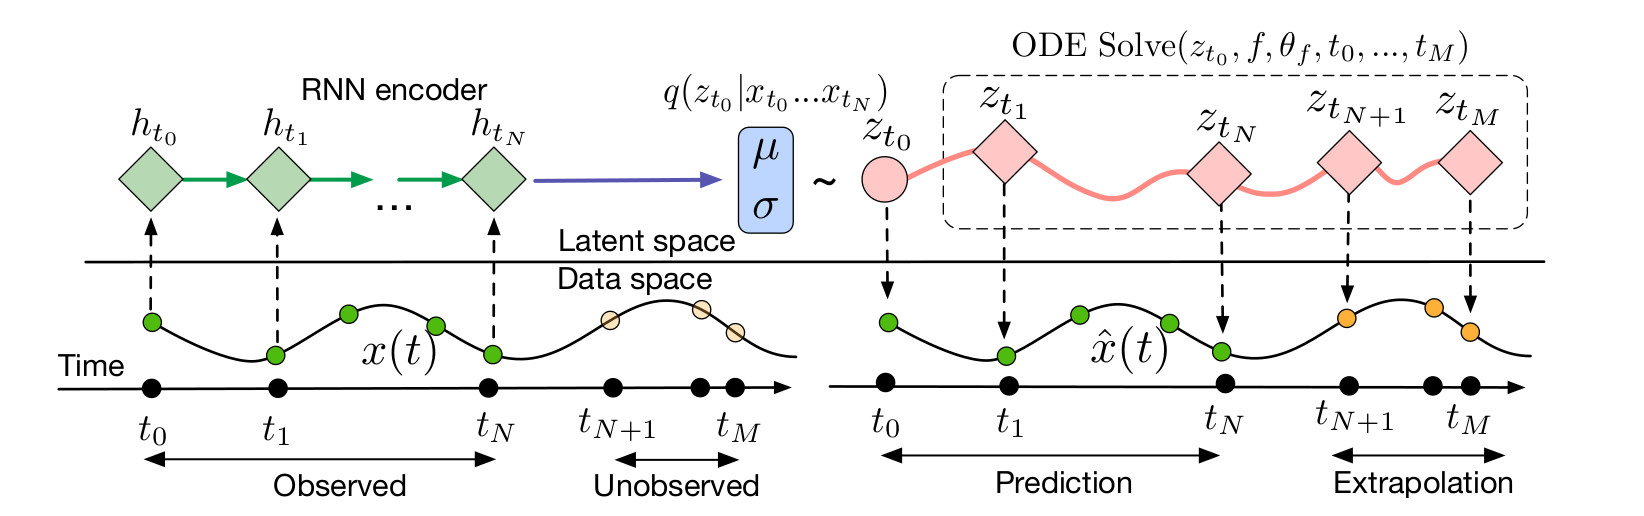
\includegraphics[width=0.9\textwidth]{/home/benjamin/Folders_Python/MVA/MVA_Stage/images/Neural_ODE_01.png}
    \caption{Latent ODE model}
    \label{fig:Latent ODE model}
\end{figure}

The model is trained maximizing a \gls{vlb} as usual. 

Here, the stochastic variables are $z_{t_0}$ and the $x_{t_i}$'s, the joint distribution writes:
\begin{align}
    p(x_{t_1:t_N}, z_{t_0}) &= p(z_{t_0})p(x_{t_1:t_N} \vert z_{t_0}) \\
    &= p(z_{t_0}) \prod_{t=1}^{N}p_{\theta_x}(x_{t_i} \vert z_{t_i})
\end{align}
And the likelihood:
\begin{align}
    p(x_{t_1:t_N}) &= \frac{p(x_{t_1:t_N}, z_{t_0})}{p(z_{t_0} \vert x_{t_1:t_N})} \\
    \log{p(x_{t_1:t_N})} &= \mathbb{E}_{q_{\phi}(z_{t_0} \vert x_{t_1:t_N})} \log{\frac{p(x_{t_1:t_N}, z_{t_0})}{q_{\phi}(z_{t_0}\vert x_{t_1:t_N})}\frac{q_{\phi}(z_{t_0}\vert x_{t_1:t_N})}{p(z_{t_0} \vert x_{t_1:t_N})}}
\end{align}
The \gls{vlb} is:
\begin{align}
    \log{p(x_{t_1:t_N})} &\geq \mathbb{E}_{q_{\phi}(z_{t_0} \vert x_{t_1:t_N})} \log{\frac{p(x_{t_1:t_N}, z_{t_0})}{q_{\phi}(z_{t_0}\vert x_{t_1:t_N})}} \\
    &= \mathbb{E}_{q_{\phi}(z_{t_0} \vert x_{t_1:t_N})} \log{\frac{p(z_{t_0}) \prod_{t=1}^{N}p_{\theta_x}(x_{t_i} \vert z_{t_i})}{q_{\phi}(z_{t_0}\vert x_{t_1:t_N})}} \\
    &= \sum_{i=1}^{N} \mathbb{E}_{q_{\phi}(z_{t_0} \vert x_{t_1:t_N})} \log{p_{\theta_x}(x_{t_i} \vert z_{t_i})} - \mathbb{KL}(q_{\phi}(z_{t_0} \vert x_{t_1:t_N}) \vert\vert p(z_{t_0}))
\end{align}
With the simple prior $p(z_{t_0}) = \mathcal{N}(0,1)$.

Optimizing the \gls{vlb} requires that we compute the gradients on $\log{p_{\theta_x}(x_{t_i} \vert z_{t_i})}$ w.r.t. $\theta_f$, as the $z_{t_i}$ are solutions of the \gls{ode} depending 
on $f$ and its set of parameters $\theta_f$. Methods to do so are: forward sensitivity, backpropragation through the \gls{ode} solver,
and the \textbf{adjoint sensitivity method} described in \cite{pontriagin_mathematical_2018}. 
(the interested reader will find a proof sketch in the appendix \ref{sec:adjoint_sensitivity_method}, 
and a full review in \cite{sengupta_efficient_2014}).

\section{Latent SDE models}

\glspl{latent ode} models have limitations :
\begin{itemize}
    \item the latent dynamic is deterministic by design
    \item the intial variable $z_{t_0}$ encompasses the entire randomness of the prior, and can become
    unnaturally large to account for randomness along the entire timeline
\end{itemize}

The idea in \cite{li_scalable_2020} is then to add some noise to the deterministic computation of the latent variable:
\begin{align}
    \frac{dz_t}{dt} &= f_{\theta_f}(z_t,t) + \epsilon_t \\
    \epsilon_t &\sim \mathcal{N}(0,Q \, \textit{Id})
\end{align}
Which leads to an \gls{sde} prior:
\begin{align}
    \label{latent sde prior}
    dZ_t &= f_{\theta}(Z_t, t)dt + \sigma_{\theta}(Z_t,t)dB_t \\
    Z_{t_0} &\sim Z_0
\end{align}
where we used $\sigma_{\theta}$ instead of our usual $L(Z_t,t)$ to stick to the notations of the paper.

\ref{latent sde prior} defines a prior distribution over functions. In order to draw a sample function, we would:
\begin{itemize}
    \item draw a sample $z_{t_0} \sim Z_0$
    \item draw a random Brownian motion $\tilde{B_t}$ path from $B_t$
    \item compute $z_t - z_{t_0} = \int_{t_0}^{t} f_{\theta}(Z_t, t)dt + \int_{t_0}^{t} \sigma_{\theta}(Z_t,t)d\tilde{B_t}$
\end{itemize}

The approximate posterior can also be described as a \gls{sde}:
\begin{align}
    dZ_t &= f_{\phi}(Z_t,t)dt + \sigma_{\phi \, = \, \theta}(Z_t,t)dB_t \\
    Z_{t_0} &= z_0 \, \text{from prior}
\end{align}
where:
\begin{itemize}
    \item the prior and the approximate posterior share the same diffusion for the $\mathbb{KL}$ to have the same support
    \item the prior and the approximate posterior have the same starting value $z_0$
\end{itemize}

We will use neural networks to learn the drift $f_{\phi}$ and the diffusion $\sigma_{\theta}$, which requires that we are able to compute the gradient of 
a functional (loss) of type:
\begin{align}
    L(\theta) &= L \left( \int_{t_0}^{t_1} f_{\theta}(Z_t, t)dt + \int_{t_0}^{t} \sigma_{\theta}(Z_t,t)dB_t \right)
\end{align}
where $\int_{t_0}^{t} \sigma_{\theta}(Z_t,t)dB_t$ is actually a random variable!

It appears that the adjoint sensitivity method can be adapted to SDEs (see \cite{li_scalable_2020}).

We reproduce the model from the paper:

\begin{figure}[H]
    \centering
    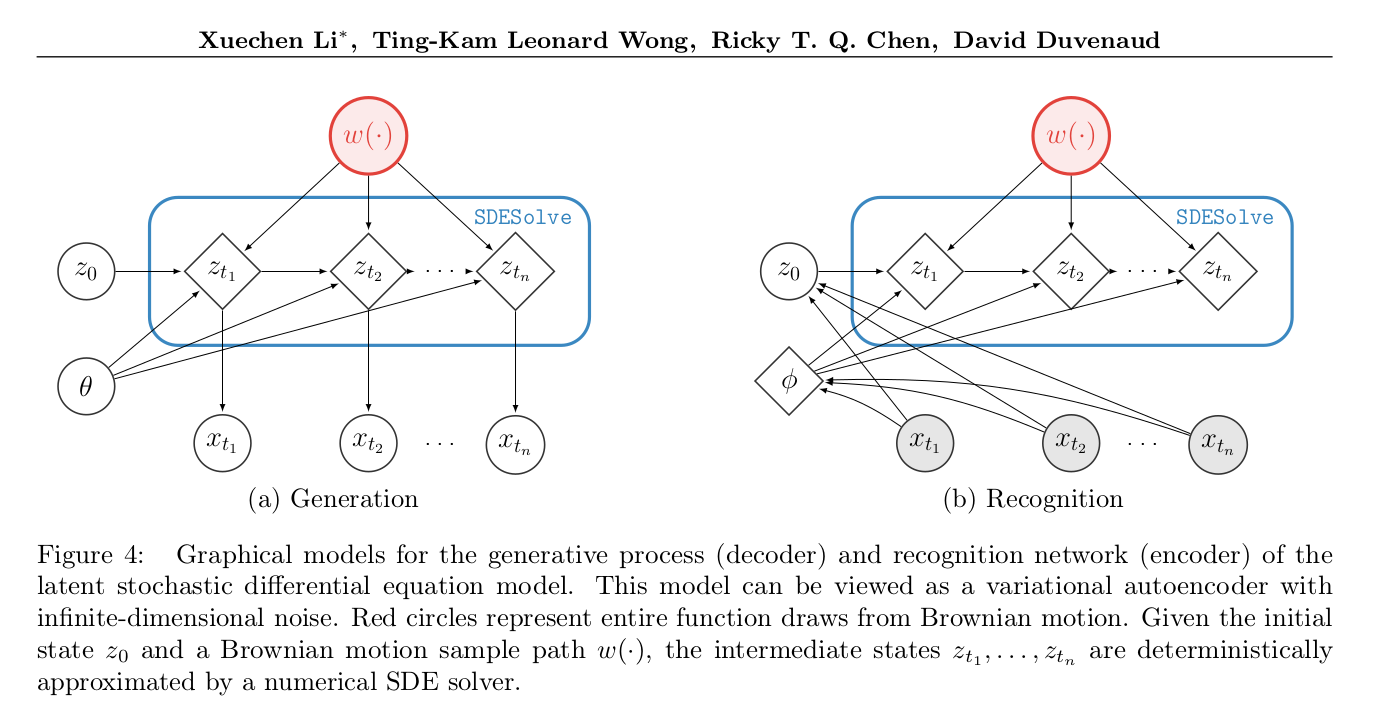
\includegraphics[width=0.9\textwidth]{/home/benjamin/Folders_Python/MVA/MVA_Stage/images/Latent_SDE_01.png}
    \caption{Latent SDE model}
    \label{fig:Latent SDE}
\end{figure}

The stochastic \gls{vlb} writes:
\begin{align}
    \mathcal{L}(\theta, \phi, x_{1:T}) &= \mathbb{E} \left(
        \frac{1}{2}\int_{0}^{T} \vert \frac{f_{\theta}(z_t,t) - f_{\phi}(z_t,t)}{\sigma_{\theta}(z_t,t)}dt \vert^{2} - 
        \sum_{i=1}^{N} \log{p_{\theta_x}}(x_{t_i} \vert z_{t_i})
        \right)
\end{align}
